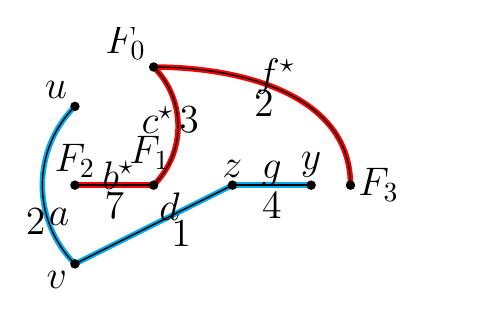
\begin{tikzpicture}[line cap=round,line join=round,x=1cm,y=1cm]
\clip(-.6,-.5) rectangle (5,3);


\draw [line width=2pt,color=cyan] (0,0) to[in=-135,out=135,looseness=1]  (0,2); % v -- u
\draw [line width=.5pt] (0,0) to[in=-135,out=135,looseness=1]  (0,2); % v -- u
%\draw [line width=1pt] (0,0) to[in=-45,out=45,looseness=1]  (0,2);   % v -- u
\draw [line width=2pt,color=cyan] (2,1) to  (0,0); % 4 -- 6
\draw [line width=.5pt] (2,1) to  (0,0); % 4 -- 6
\draw [line width=2pt,color=cyan] (2,1) to  (3,1); % 4 -- 6
\draw [line width=.5pt] (2,1) to  (3,1); % 4 -- 6
%\draw [line width=1pt] (2,1) to  (0,2); % 4 -- 6
%\draw [line width=1pt] (2,1.05) to[out=45,in=-45,looseness=50] (2,.95); % 4 -- 4

\draw [line width=2pt,color=red] (1,2.5) to[out=-45,in=45,looseness=1] (1,1); % F0 -- F1
\draw [line width=.5pt] (1,2.5) to[out=-45,in=45,looseness=1] (1,1); % F0 -- F1
%\draw [line width=1pt] (1,2.5) to[out=20,in=-70,looseness=10] (1,1); % F0 -- F1
%\draw [line width=1pt] (1,2.5) to[out=170,in=180,looseness=2.5] (0,1); % F0 -- F2
\draw [line width=2pt,color=red] (1,2.5) to[out=0,in=90,looseness=1] (3.5,1); % F0 -- F3
\draw [line width=.5pt] (1,2.5) to[out=0,in=90,looseness=1] (3.5,1); % F0 -- F3
\draw [line width=2pt,color=red] (1,1) to (0,1); % F1 -- F2
\draw [line width=.5pt] (1,1) to (0,1); % F1 -- F2

\begin{scriptsize}
\draw [fill=black] (0,2) circle (1.5pt);
\draw (0,2) node[anchor=south east] {{\Large $u$}};


\draw [fill=black] (0,0) circle (1.5pt);
\draw (0,0) node[anchor=north east] {{\Large $v$}};
\draw [fill=black] (2,1) circle (1.5pt);
\draw (2,1) node[anchor=south] {{\Large $z$}};
\draw [fill=black] (3,1) circle (1.5pt);
\draw (3,1) node[anchor=south] {{\Large $y$}};


\draw [fill=black] (1,2.5) circle (1.5pt);
\draw (1,2.5) node[anchor=south east] {{\Large $F_0$}};
\draw [fill=black] (1,1) circle (1.5pt);
\draw (.95,1.1) node[anchor=south] {{\Large $F_1$}};
\draw [fill=black] (0,1) circle (1.5pt);
\draw (0,1) node[anchor=south] {{\Large $F_2$}};
\draw [fill=black] (3.5,1) circle (1.5pt);
\draw (3.5,1) node[anchor=west] {{\Large $F_3$}};


\draw (-0.2,.8) node[anchor=north] {{\Large $a$}};
\draw (-0.5,.8) node[anchor=north] {{\Large $2$}};

\draw (0.55,1.4) node[anchor=north] {{\Large $b^\star$}};
\draw (0.5,1) node[anchor=north] {{\Large $7$}};

\draw (1.05,2.1) node[anchor=north] {{\Large $c^\star$}}; % u -- w
\draw (1.45,2.1) node[anchor=north] {{\Large $3$}}; % u -- w

\draw (1.2,1) node[anchor=north] {{\Large $d$}}; % v -- w
\draw (1.35,.65) node[anchor=north] {{\Large $1$}}; % v -- w

\draw (2.5,1.4) node[anchor=north] {{\Large $g$}}; % v -- w
\draw (2.5,1) node[anchor=north] {{\Large $4$}}; % v -- w

\draw (2.55,2.7) node[anchor=north] {{\Large $f^\star$}}; % w -- w
\draw (2.4,2.3) node[anchor=north] {{\Large $2$}}; % w -- w

\end{scriptsize}
\end{tikzpicture}
